\section{Filmkeresés és film oldal}

A filmkeresés az alkalmazás egyik nyilvánosan elérhető funkciója. A keresőmező a navigációs sávban található, így a felhasználó az alkalmazás bármely részéről indíthat keresést. Enter lenyomásakor a kliensoldali navigáció a \texttt{/search} útvonalra irányít, ahol a keresett kifejezés query paraméterként jelenik meg.

A keresőoldal szerveroldali komponensként működik. Az oldal a \texttt{searchParams} alapján kiolvassa a keresési kifejezést és az aktuális oldalszámot, majd a \texttt{searchMovies} függvényen keresztül lekéri a TMDB találatait. A válaszban érkező adatokat az alkalmazás normalizált formában használja, ezért a felületen már egységes mezőnevek jelennek meg, például \texttt{posterPath}, \texttt{releaseDate} és \texttt{voteAverage}.

A találatok megjelenítését külön \texttt{SearchResultCard} komponens végzi. A kártya a film plakátját, címét, megjelenési évét, rövid leírását és TMDB értékelését mutatja. Ha egy filmhez nem érhető el plakát vagy leírás, a komponens helyettesítő állapotot jelenít meg, így a felület hiányos külső API-adatok esetén is használható marad. A találati lista lapozását a \texttt{PaginationButtons} komponens kezeli.

\begin{figure}[H]
    \centering
    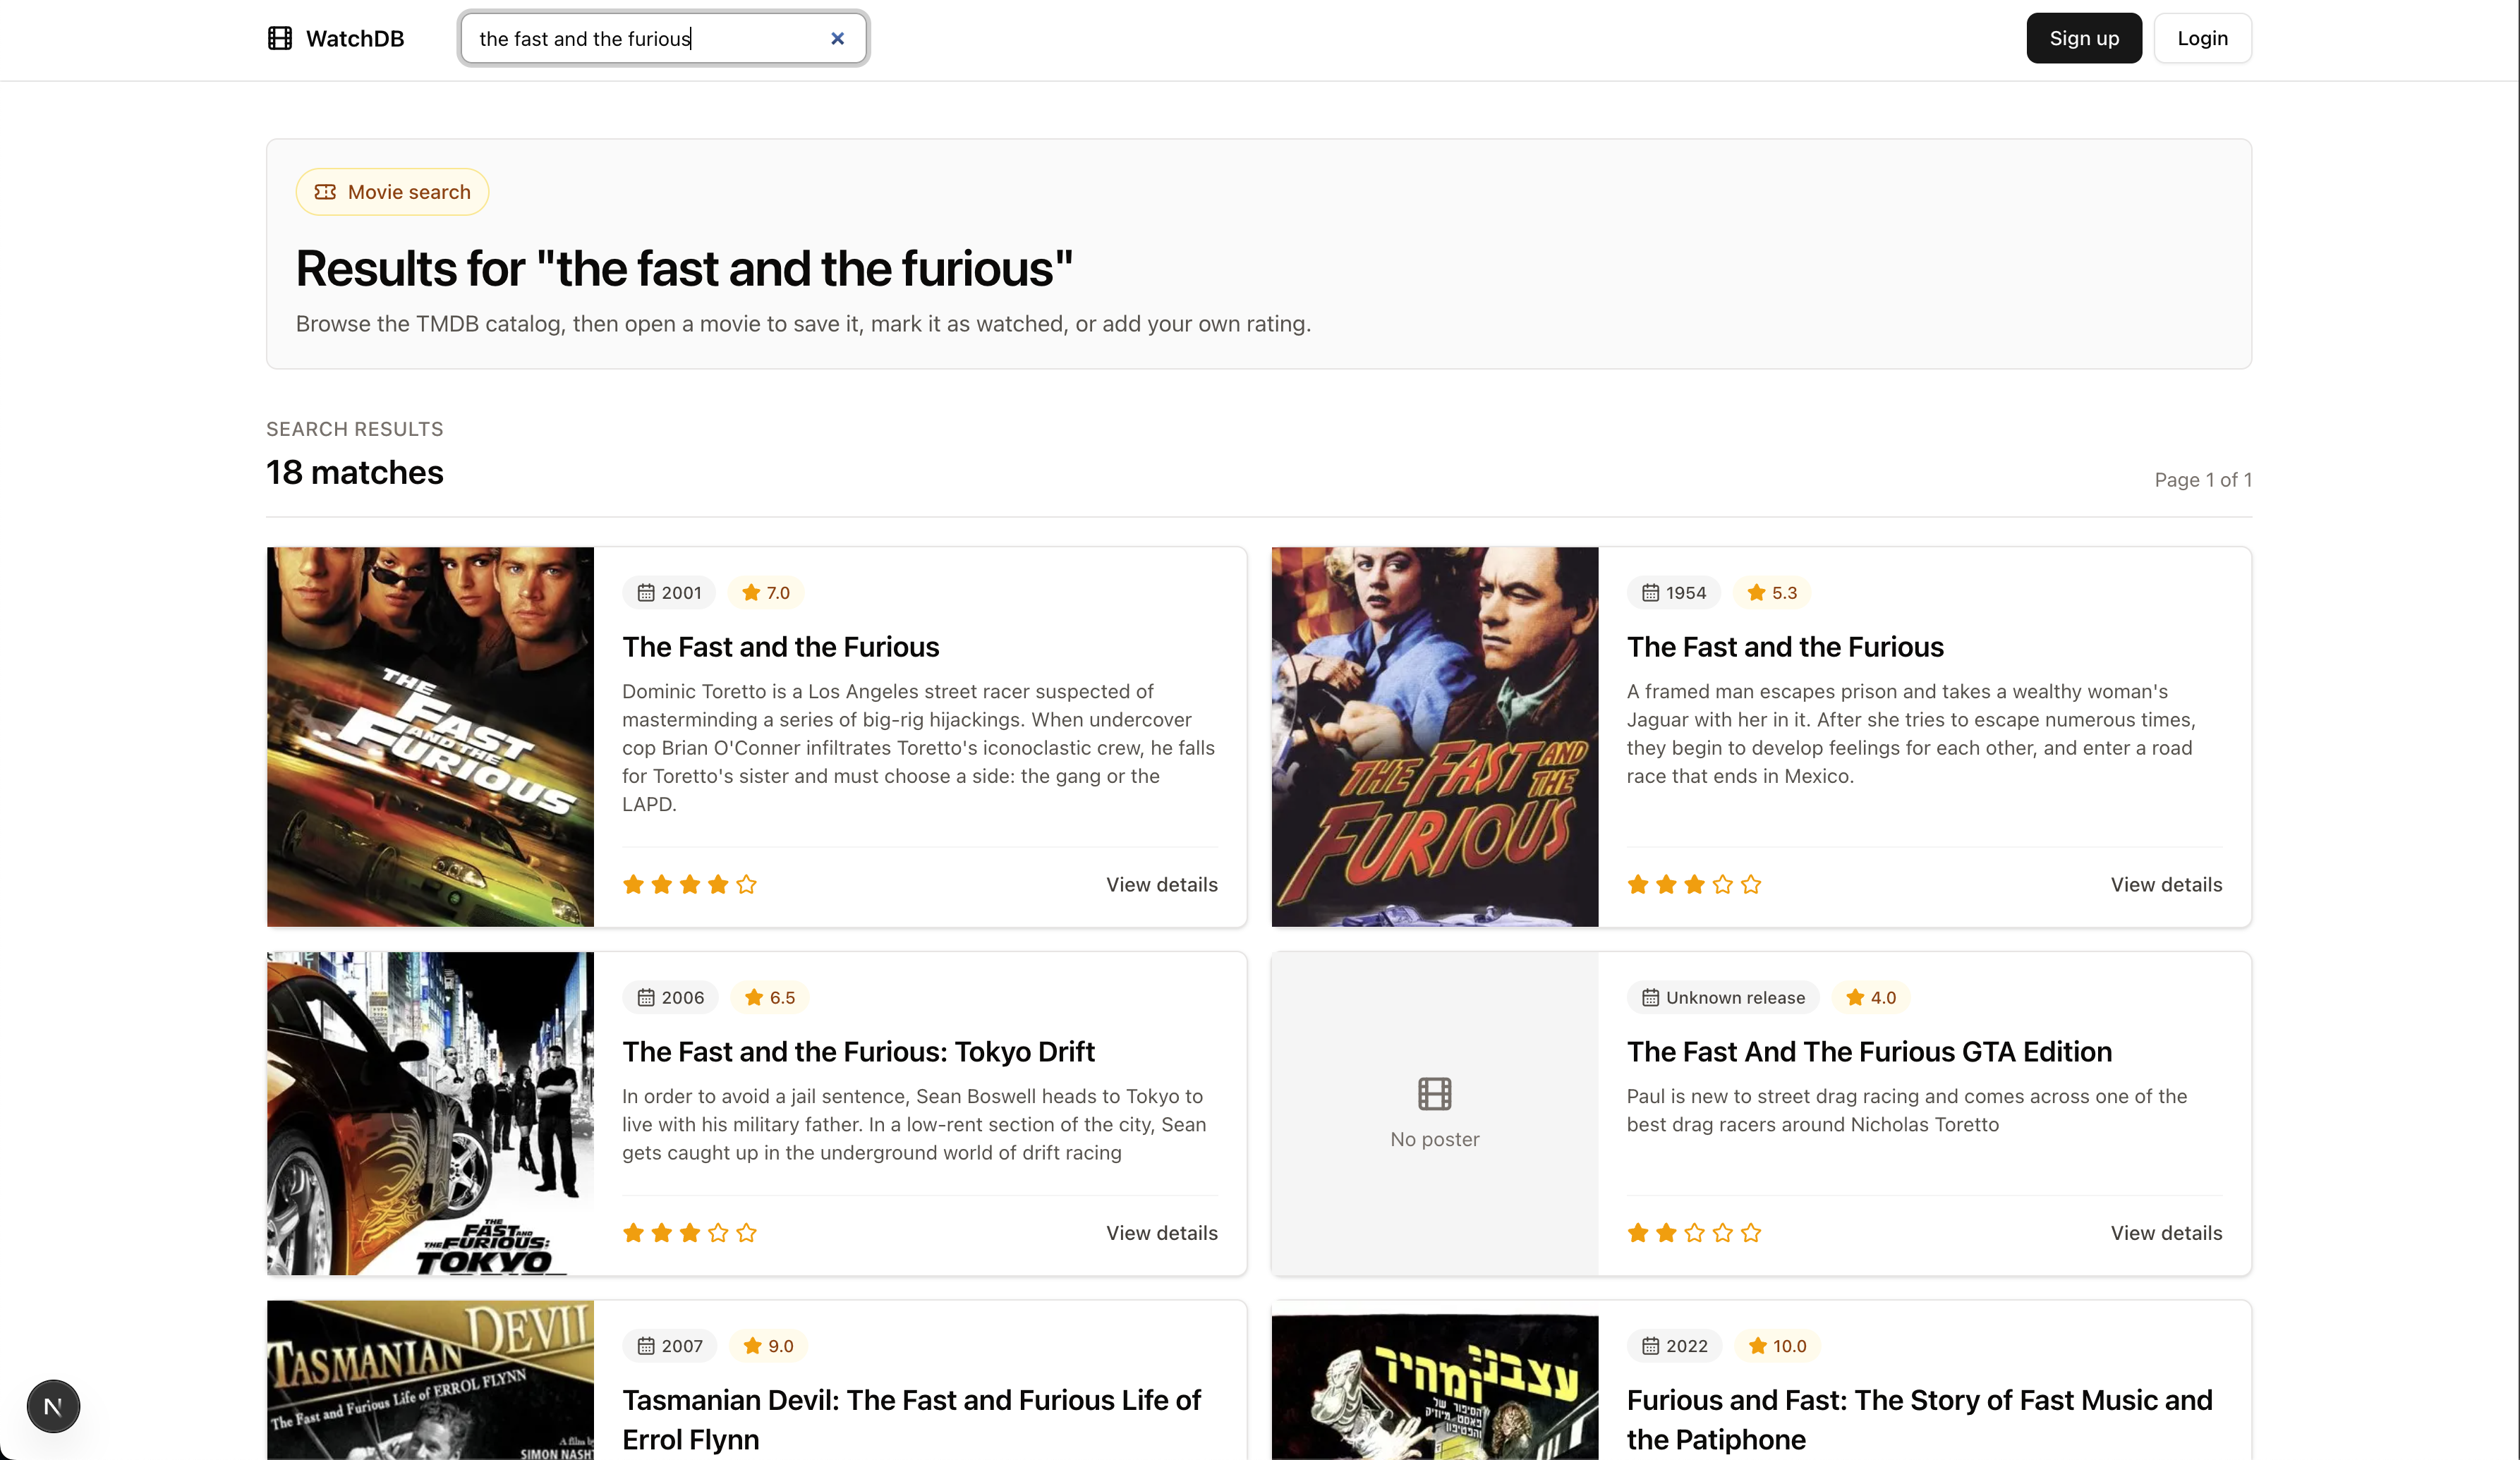
\includegraphics[width=0.85\textwidth]{chapters/chapter-6-implementation/search-page.png}
    \caption{A filmkeresési találatok megjelenítése}
    \label{fig:watchdb-search-page}
\end{figure}

A film oldal a \texttt{/movies/[id]} dinamikus útvonalon érhető el. Az oldal először számmá alakítja az URL-ben érkező azonosítót, majd hibás azonosító vagy sikertelen adatlekérés esetén a Next.js \texttt{notFound} függvényével kezeli a hibás állapotot. Sikeres lekérés esetén a \texttt{getMovieDetails} függvény tölti be a filmhez tartozó részletes adatokat.

A film oldal felső része a \texttt{MovieDetailHero} komponensben jelenik meg. Ez tartalmazza a háttérképet, a plakátot, a címet, a műfajokat, a rendezőket, a játékidőt és a TMDB értékelést. Ugyanitt találhatók a műveletek gombjai is, például a watchlisthez adás és a megnézettként jelölés. Az oldal alsó része az áttekintést, a főbb szereplőket és az alapvető metaadatokat jeleníti meg.

\begin{figure}[H]
    \centering
    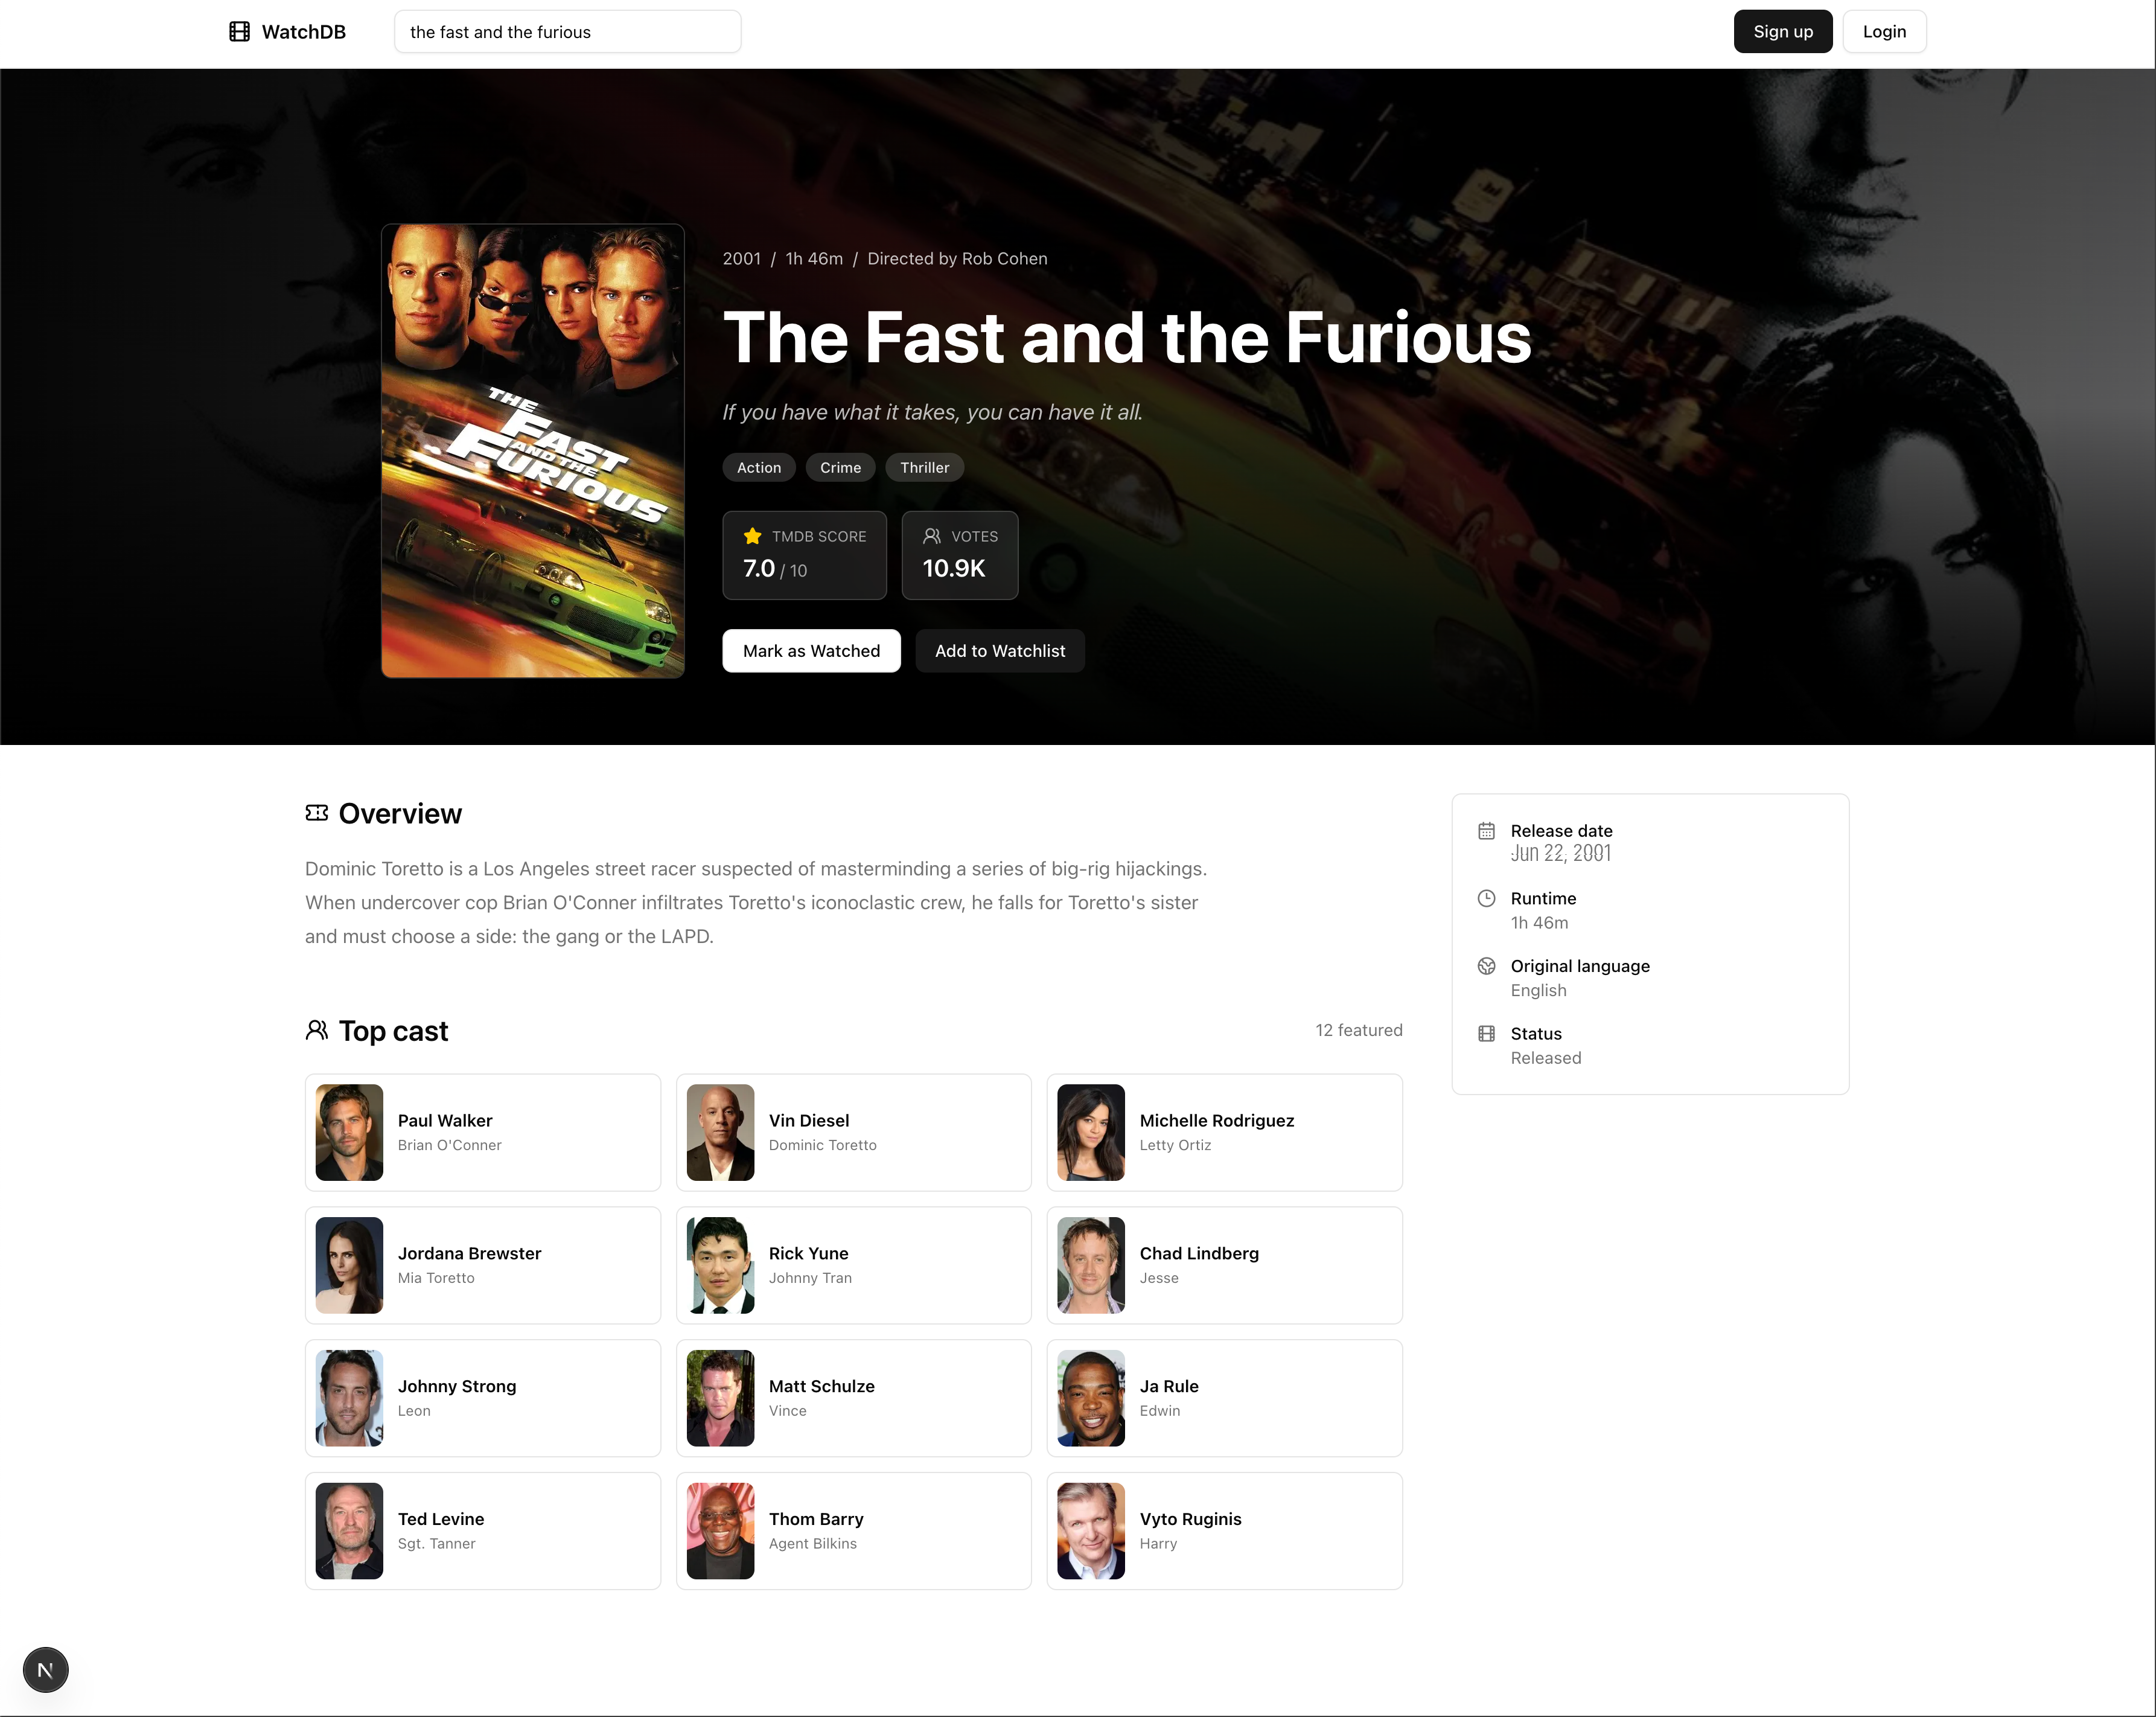
\includegraphics[width=0.85\textwidth]{chapters/chapter-6-implementation/movie-detail-page.png}
    \caption{A film oldal felépítése}
    \label{fig:watchdb-movie-detail-page}
\end{figure}
